\subsection{Research Context}

As explained in the previous section (Section \ref{Sec: Literature Review}), the VQA approach to circuit design for QNN construction overcomes many constraints of static quantum circuits. Most importantly, it allows the construction of trainable circuits, which support the development of practical applications in optimisation and machine learning.
However, we have observed the existence of barren plateaus, causing the variance of the cost function gradient to vanish exponentially with the number of qubits.
We have thus investigated three methods to mitigate this phenomenon, i.e. by using a local cost function with shallow circuits, by relying on the identity block and by utilising layerwise learning \cite{cerezoCostFunctionDependent2021, liuParameterInitializationMethod2021, skolikLayerwiseLearningQuantum2021}.

In the following sections, we will describe an approach to evaluating these three methods, and at the same time outline an approach to answering the study research question (see Section \ref{Problem Section}). This will be done by conducting a series of experiments such that different methods could be applied to the object of this study.
This process is known as \emph{technology-oriented empirical research} \cite[sect 2.4]{wohlinExperimentationSoftwareEngineering2012}.

We summarise the adopted research process in Figure \ref{Research Activities Figure}.
Our main objects and the different technical treatments for the experiment are discussed in section \ref{Objects section}, the two phases of the experiment in section \ref{Research Activities section}, and finally the confirmation of results from the experiment in section \ref{Data Collecting Section}.

\begin{figure}
    \centering
    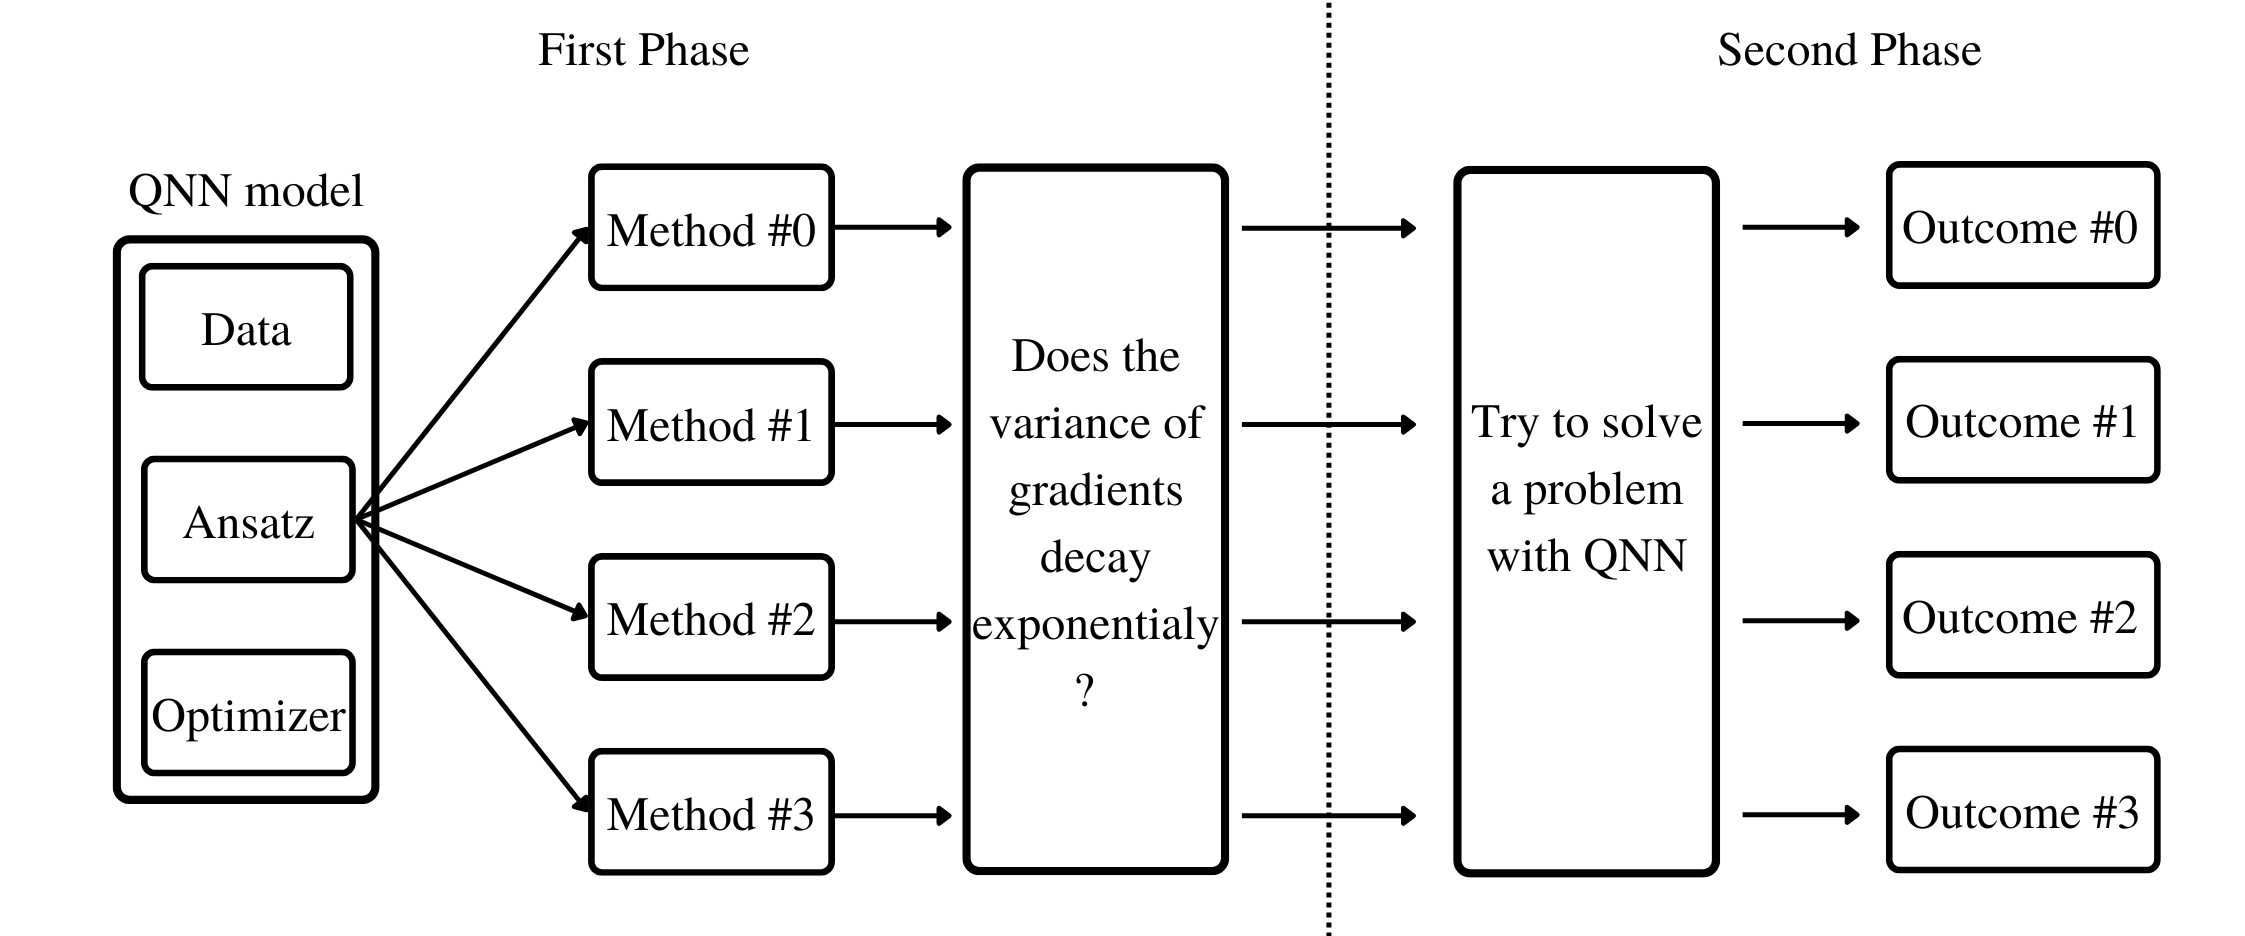
\includegraphics[width=\linewidth]{./ResearchDesign/Appendices/ExperimentDiagram.png}
    \caption{
        The adopted research process.
    }
    \label{Research Activities Figure}
\end{figure}
